\documentclass{IEEEtran}

\usepackage[utf8]{inputenc}
\usepackage{graphicx}
\usepackage{amsmath}
\usepackage{siunitx}
\usepackage{listings}
\usepackage[citestyle=ieee,sorting=none,bibencoding=utf8,backend=biber]{biblatex}
%\usepackage{caption}
\usepackage{subcaption}
\usepackage{tabularx}
\usepackage{booktabs}
\usepackage{physics}

\usepackage{algorithm}
\usepackage[noend]{algpseudocode}

\graphicspath{{images/}}
\bibliography{bibliography}
\makeatletter
\def\BState{\State\hskip-\ALG@thistlm}
\makeatother

\author{J.R. Powers-Luhn}
\title{Anomaly Detection}
\date{November 8th, 2018}

\begin{document}
\maketitle

\begin{abstract}

Principal component analysis is employed as a mechanism to detect outlier measurements from temperature and sightglass level readings in a Slurry Red Ceramic Melter. Two statistical metrics are employed to detect outliers: Hotelling's $T^2$ and the $Q$-statistic. The process of setting thresholds for these statistics is discussed and a brief exploration of the use of these statistics in diagnostics is offered.

\end{abstract}

\section{Introduction}

Interrelated process failures fall into two categories. The failure can be within the model (meaning that the measured values are within the normal bounds in which the model was trained but do not follow the established relationships) or outside of the model (meaning that there is variation that cannot be explained by the model). A well designed fault detection system should be able to identify each of these types of faults.

Two statistics that can be used to detect these types of faults are Hotelling's $T^2$ (for detecting variation within a model) and $Q$-statistics (for detecting deviation from a model). These statistics measure deviation by using a principal component analysis transformation then calculating the deviation from the model. Simple thresholds can be set using known training data. Values that then exceed these thresholds can trigger alarms or investigation of the instruments that produced the measurements. Further, it is possible to calculate the relative contribution from each measurement in a data point to the $T^2$ and $Q$ statistic, assisting in diagnostics.

\section{Methodology}

In order to measure a measurement's deviation within a model, Hotelling's $T^2$ (equation \ref{eq:t2}) statistic is used. A generalization of the student's T-test, this measures how far the measurement has departed from the center of the principal component space. 

\begin{equation}
T^2_i = t_i \lambda^-1 t_i^T
\label{eq:t2}
\end{equation}

If there is variation outside of the model the residuals will be high. This is captured by a second statistic: the $Q$ statistic (equation \ref{eq:q}), which measures deviation outside the model.

\begin{equation}
Q_i = x_i ( \mathbf{I} - \mathbf{P}_k \mathbf{P}_k^T ) x_i^T
\label{eq:q}
\end{equation}

The values of these statistics, calculated on a ``known good'' training set, can be used to set alarm thresholds for future data.

A PCA model was generated using a training data set of 450 samples of 21 values each. The number of principal components included in the model was determined by increasing the number of components and calculating the $T^2$ and $Q$ statistics. After two PC's were included the $T^2$ values did not change and the $Q$ statistics were reduced by an order of magnitude. Adding additional components did continue to lower as more components were added, but the rate decreased significantly--the next order-of-magnitude reduction threshold was not reached until 9 PC's were included.  A threshold was set based on the 95\% quantile of the data, giving values of \num{289} for $T^2$ and \num{16.3} for $Q$. Two test data sets were then projected into the same PC space and data points with $T^2$ and $Q$ values above the selected thresholds were identified.

\section{Results}

$T^2$ and $Q$ statistics for the training data are shown in figure \ref{fig:data_q_and_t2}. A model employing two principal components was selected, producing 95\% quantile thresholds of \num{289} for $T^2$ and \num{16.3} for $Q$.

\begin{centering}
\begin{figure}
\centering
\begin{center}
	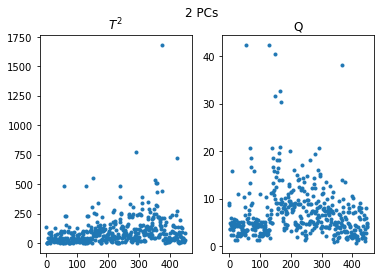
\includegraphics[width=0.48\textwidth]{data_q_and_t2}
	\caption{$Q$ and $T^2$ statistics for selected PCA model. After 2
			 \label{fig:data_q_and_t2}}
\end{center}
\end{figure}
\end{centering}

The same transformation and thresholds were applied to the test1 and test2 datasets. Scatterplots of the two principal component scores were plotted against each other. The test1 data (figure \ref{fig:test1_scatter}) essentially fit that model, with only a few values (identified in orange) exceeding the thresholds set.

\begin{figure}[t!]
    \centering
    \begin{subfigure}[t]{0.48\linewidth}
        \centering
        \includegraphics[width=\linewidth]{{test1_t2}.png}
        \caption{$T^2$ statistic}
    \end{subfigure}%
    ~ 
    \begin{subfigure}[t]{0.48\linewidth}
        \centering
        \includegraphics[width=\linewidth]{{test1_q}.png}
        \caption{Q-statistic}
    \end{subfigure}
    \caption{test1 data principal components plotted against each other. Only three scattered points exceed the $T^2$ threshold, while five exceed the $Q$ threshold (identified in orange). This is consistent with the training dataset.}
    \label{fig:test1_scatter}
\end{figure}

The contribution of each variable to the high $T^2$ score was calculated. In the case of the first outlier no unusual contribution was noted, meaning that it might be the result of normal statistical fluctuation. The second outlier had relatively large contributions from the \numlist{17;19}th measurements. Finally the last outlier had a large contribution from the 5th measurement. These instruments should be examined for potential failure.

A similar analysis was applied to the $Q$ statistics for the five outliers in that parameter. Few measurements stood out except in the case of the first outlying point which showed significant deviation in the 9th measurement and smaller (though still significant) deviation in the 19th. Again, these instruments and portions of the process should be examined more closely to search for a fault.

The test2 data, on the other hand, deviated significantly from the model (figure \ref{fig:test2_scatter}). The $Q$-statistic value for nearly every one of the points exceeded the threshold and a large number of the points also exceeded their threshold. Extracting diagnostic information from these measurements would be difficult; the entire system should be examined.

\begin{figure}[t!]
    \centering
    \begin{subfigure}[t]{0.48\linewidth}
        \centering
        \includegraphics[width=\linewidth]{{test2_t2}.png}
        \caption{$T^2$ statistic}
    \end{subfigure}%
    ~ 
    \begin{subfigure}[t]{0.48\linewidth}
        \centering
        \includegraphics[width=\linewidth]{{test2_q}.png}
        \caption{Q-statistic}
    \end{subfigure}
    \caption{test2 data principal components plotted against each other. Many of the points exceed the $T^2$ threshold; nearly all of them exceed the $Q$ threshold.}
    \label{fig:test2_scatter}
\end{figure}

\section{Conclusions}

A PCA method for detecting anomalies in data was examined employing two statistical measures--Hotelling's $T^2$ and the $Q$-statistic. Thresholds were set for these statistics and were applied to two sets of data containing anomalies. In the first case, it was possible to extract information as to the source of anomalous readings, potentially assisting the diagnostic process. In the second case it was quickly apparent that the model no longer described the data and that the entire model should be re-examined from scratch. 

\onecolumn
\section{Appendix}
Python code used to perform calculations and generate graphics.
\lstset{frame=single}
\lstinputlisting[language=Python]{HW08.py}

\end{document}